\subsection{Optimizations for Leiden algorithm}
\label{sec:leiden}

We extend our optimization techniques, originally designed for the Louvain method \cite{sahu2023gvelouvain}, to the Leiden algorithm. Specifically, we implement an \textit{asynchronous} version of the Leiden algorithm, allowing threads to operate independently on distinct sections of the graph. While this approach promotes faster convergence, it also introduces variability into the final result \cite{com-shi21}. To ensure efficient computations, we allocate a dedicated hashtable per thread. These hashtables serve two main purposes: they keep track of the delta-modularity associated with moving to each community connected to a vertex during the local-moving/refinement phases, and they record the total edge weight between super-vertices in the aggregation phase of the algorithm \cite{sahu2023gvelouvain}.

Our optimizations encompass several strategies, including utilizing OpenMP's \textit{dynamic} loop scheduling, capping the number of iterations per pass at $20$, employing a tolerance drop rate of $10$ (threshold scaling), initiating with a tolerance of $0.01$, using an aggregation tolerance of $0.8$ to avoid performing aggregations of minimal utility, implementing flag-based vertex pruning (instead of a queue-based one \cite{nguyenleiden}), utilizing parallel prefix sum, and using preallocated Compressed Sparse Row (CSR) data structures for identifying community vertices and storing the super-vertex graph during aggregation. Additionally, we employ fast collision-free per-thread hashtables, well separated in their memory addresses \cite{sahu2023gvelouvain}.

We attempt two approaches of the Leiden algorithm. One uses a \textit{greedy refinement phase} where vertices greedily optimize for delta-modularity (within their community bounds), while the other uses a \textit{randomized refinement phase} (using fast \textit{xorshift32} random number generators), where the likelihood of selection of a community to move to (by a vertex) is proportional to its delta-modularity, as originally proposed \cite{com-traag19}. Our results, shown in Figures \ref{fig:leidenopt-runtime} and \ref{fig:leidenopt-modularity}, indicate the \textit{greedy approach} performs the best on average, both in terms of runtime and modularity. We also try medium and heavy variants for both approaches, which disables threshold scaling and aggregation tolerance (including threshold scaling) respectively, However, we do not find them to perform well overall.\ignore{On \textit{europe\_osm} graph, our parallel Greedy-Leiden (which we from here on refer to simply as Leiden) runs $3\times$ faster than Nguyen \cite{nguyenleiden}.}

\ignore{We fixed a bug that caused the Leiden algorithm to fail in finding communities on road networks and kmer graphs. The issue was forgetting to reset the affected vertices flags before running the refinement phase.}




\subsubsection{Implementation details}

We use a top-level parallel block, OpenMP's dynamic loop scheduling (with a chunk size of $2048$) along with \verb|nowait| directive, and a single shared rank vector to implement our \textit{Barrier-free} PageRank. Dynamic loop scheduling causes each running thread obtains a chunk of vertices to be processed from a global work pool, resulting in the running threads to have a balanced workload. This also enables our algorithm to be fault-tolerant to random thread delays and crashes (in the crash-stop model).




\subsection{Our Naive-dynamic Barrier-free PageRank (\NaiBarf{})}
\label{sec:naive}

As discussed previously, the \textit{Naive-dynamic} approach is a simple method for updating vertex ranks in dynamic networks by initializing them with ranks from the previous snapshot. We apply this approach to our improved \textit{Barrier-free} PageRank (shown in Algorithm \ref{alg:barrier-free-naive-dynamic}), and refer to it as \NaiBarf{}. We also include the pseudocode for \textit{Naive-dynamic With-barrier} PageRank (\NaiWbar{}) for reference in Algorithm \ref{alg:with-barrier-naive-dynamic}.

% \input{src/alg-barrier-free-naive-dynamic}
% \input{src/alg-with-barrier-naive-dynamic}




\subsection{Our Dynamic Traversal Barrier-free PageRank (\TraBarf{})}
\label{sec:traversal}

The \textit{Dynamic Traversal} approach (as discussed in Section \ref{sec:about-traversal}) marks all vertices reachable from every vertex involved in edge deletions or insertions as affected. In our barrier-free implementation of this approach (shown in Algorithm \ref{alg:barrier-free-dynamic-traversal}), which we refer to as \TraBarf{}, we allow any thread to start computing ranks as soon as it has finished marking affected vertices (based on edge updates assigned to it). Additionally, we provide the pseudocode for \textit{Dynamic Traversal With-barrier} PageRank (\TraWbar{}), which can be referred to in Algorithm \ref{alg:with-barrier-dynamic-traversal}.
% A simple dynamic algorithm works as follows. Set $\pr^t(v)$ to $\pr^{t-1}(v)$ for all nodes $v$, and run Algorithm CalculateRanks on $G^t$. This algorithm, which we label as Algorithm Naive-PageRank-BarrierFree. In other words, this simple approach does not distinguish vertices that are likely have a change in their pagerank values to those that do not have a change in their pagerank. 

However, our experiments show that the \textit{Dynamic Traversal} approach does not perform better than the \textit{Naive-dynamic} approach for any batch size. The overhead of this approach, due to several traversals required to identify the affected vertices, limits the performance of this approach.

% \input{src/alg-barrier-free-dynamic-traversal}
% \input{src/alg-with-barrier-dynamic-traversal}




\subsection{Our Dynamic Frontier approach}
\label{sec:frontier}

The \textit{Naive-dynamic} approach processes all vertices in the graph until convergence. However, if a batch update $\Delta^{t-} \cup \Delta^{t+}$ is small compared to the total number of edges $|E|$, then it is expected that the ranks of only a few vertices change. Our proposed \textit{Dynamic Frontier} approach incorporates this aspect, and identifies affected vertices efficiently via an incremental process. We apply this approach to \textit{With-barrier} and \textit{Barrier-free} PageRank in Algorithms \ref{alg:with-barrier} and \ref{alg:barrier-free}, which we also denote as \FroWbar{} and \FroBarf{} respectively.


\subsubsection{Explanation of the approach}
\label{sec:frontier-explanation}

Consider a batch update consisting of edge deletions $(u, v) \in \Delta^{t-}$ and insertions $(u, v) \in \Delta^{t+}$. We first initialize the rank of each vertex to that obtained in the previous snapshot of the graph.

\begin{figure*}[hbtp]
  \centering
  \subfigure[Initial graph]{
    \label{fig:about-df-01}
    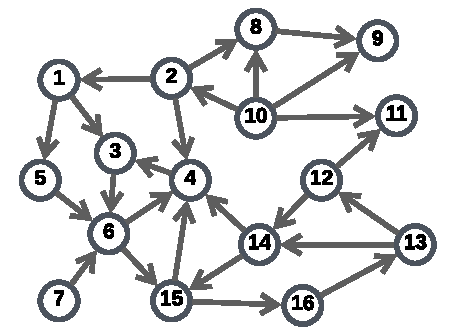
\includegraphics[width=0.23\linewidth]{out/about-df-01.pdf}
  }
  \subfigure[Marking affected (initial)]{
    \label{fig:about-df-02}
    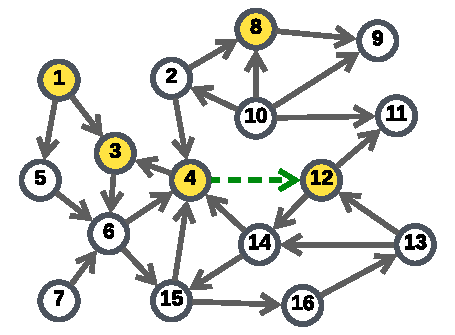
\includegraphics[width=0.23\linewidth]{out/about-df-02.pdf}
  }
  \subfigure[After first iteration]{
    \label{fig:about-df-03}
    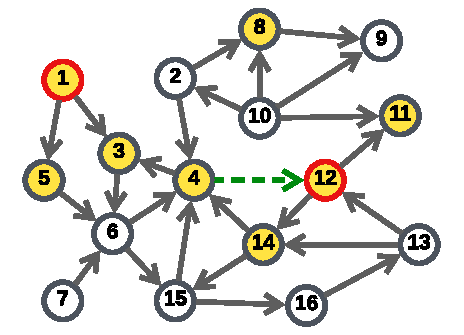
\includegraphics[width=0.23\linewidth]{out/about-df-03.pdf}
  }
  \subfigure[After second iteration]{
    \label{fig:about-df-04}
    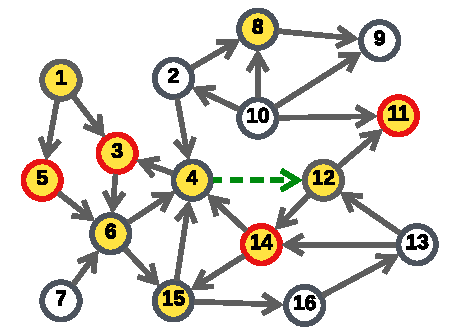
\includegraphics[width=0.23\linewidth]{out/about-df-04.pdf}
  } \\[-2ex]
  % \subfigure[]{
  %   \label{fig:about-df-05}
  %   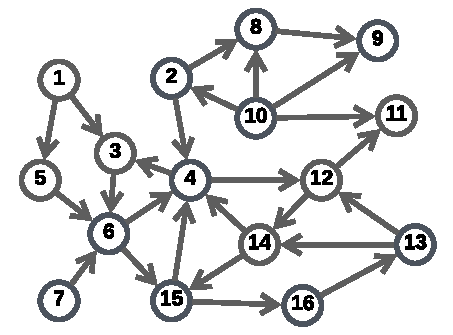
\includegraphics[width=0.18\linewidth]{out/about-df-05.pdf}
  % }
  \caption{Illustration of the \textit{Dynamic Frontier} approach through a specific example. The initial graph consists of $16$ vertices and $25$ edges. The graph is then updated with an edge insertion $(4, 12)$, and an edge deletion $(2, 1)$. Accordingly, the outgoing neighbors of vertices $4$ ($3$ and $12$) and $2$ ($1$, $4$, and $8$) are marked as affected (shown with yellow fill). When the ranks of these affected vertices are computed in the first iteration, it is found that change in rank of vertices $1$ and $12$ exceeds the frontier tolerance $\tau_f$ (shown with red border). Thus, outgoing neighbors of vertices $1$ ($3$ and $5$) and $12$ ($11$ and $14$) are also marked as affected. In the second iteration, the change in rank of vertices $3$, $5$, $11$, and $14$ is greater than $\tau_f$ --- thus their outgoing vertices are marked as affected. In the subsequent iteration, the ranks of affected vertices are again updated. If the change in rank of every vertex is within (iteration) tolerance $\tau$, the ranks of vertices have converged, and the algorithm terminates.}
  \label{fig:about-df}
\end{figure*}


\paragraph{Initial marking of affected vertex on edge deletion/insertion:}

For each edge deletion/insertion $(u, v)$, we initially mark the outgoing neighbors of the vertex $u$ in the previous $G^{t-1}$ and current graph snapshot $G^t$ as affected (lines \ref{alg:with-barrier--mark-begin}-\ref{alg:with-barrier--mark-end} in Algorithm \ref{alg:with-barrier}, and lines \ref{alg:barrier-free--mark-begin}-\ref{alg:barrier-free--mark-end} in Algorithm \ref{alg:barrier-free}).

\paragraph{Incremental marking of affected vertices upon change in rank of a given vertex:}

Next, while performing PageRank computation (lines \ref{alg:with-barrier--compute-begin}-\ref{alg:with-barrier--compute-end} in Algorithm \ref{alg:with-barrier}, and lines \ref{alg:barrier-free--compute-begin}-\ref{alg:barrier-free--compute-end} in Algorithm \ref{alg:barrier-free}), if the rank of any affected vertex $v$ changes in an iteration by an amount greater than the \textit{frontier tolerance} $\tau'$, we mark its outgoing neighbors as affected (lines \ref{alg:with-barrier--remark-begin}-\ref{alg:with-barrier--remark-end} in Algorithm \ref{alg:with-barrier}, and lines \ref{alg:barrier-free--remark-begin}-\ref{alg:barrier-free--remark-end} in Algorithm \ref{alg:barrier-free}). This process of marking vertices continues in every iteration.

% \input{src/alg-with-barrier}
% \input{src/alg-barrier-free}


\subsubsection{A simple example}

Figure \ref{fig:about-frontier} shows an example of the \textit{Dynamic Frontier} approach. The original graph, shown in Figure \ref{fig:about-frontier-01} consists of $16$ vertices. Subsequently, Figure \ref{fig:about-frontier-02} shows a batch update applied to the original graph involving the deletion of an edge from vertex $2$ to $1$ and the insertion of an edge from vertex $4$ to $12$. Following the batch update, we perform the initial step of the \textit{Dynamic Frontier} approach, marking outgoing neighbors of $2$ and $4$ as affected, i.e., $1$, $3$, $4$, $8$, and $12$ are marked as affected. Note that vertex $2$ is not affected as it is a source of the change while vertex $4$ being a neighbour of $2$ is also affected. Now, we are ready to execute the first iteration of PageRank algorithm.

During the first iteration (see Figure \ref{fig:about-frontier-03}), the ranks of affected vertices are updated. Consider that the change in rank of vertices $1$ and $12$ is observed to be greater than frontier tolerance $\tau'$, shown with red border in Figure \ref{fig:about-frontier-03}. In response to this, the \textit{Dynamic Frontier} approach incrementally marks the outgoing neighbors of $1$ and $12$ as affected, specifically vertices $5$, $11$, and $14$.

During the second iteration (see Figure \ref{fig:about-frontier-04}), the ranks of affected vertices are again updated. Further, consider that the change in rank of vertices $3$, $5$, $11$, and $14$ is observed to be greater than frontier tolerance $\tau'$, shown with red border in Figure \ref{fig:about-frontier-03}. As before, we mark the outgoing neighbors of $3$, $5$, $11$, and $14$ as affected, namely vertices $4$, $6$, and $15$.

In the subsequent iteration, the ranks of affected vertices are again updated. If the change in rank of every vertex is within (iteration) tolerance $\tau$, the ranks of vertices have converged, and the algorithm terminates.




\subsection{Dynamic Frontier With-barrier PageRank (\FroWbar{})}
\label{sec:frontier-withbarrier}

As mentioned in Section \ref{sec:withbarrier}, we perform a synchronous rank computation with \FroWbar{} using two rank vectors $R$, and $R_{new}$ (see Algorithm \ref{alg:with-barrier}).

\paragraph{Tracking affected vertices:}

To track vertices that are marked as affected due to the current batch update $\Delta^{t-} \cup \Delta^{t+}$, we use a flag vector $V_A$ (an 8-bit integer vector).

\paragraph{Detecting convergence:}

Note that $\Delta r$ represents the change in rank of single vertex, and $\Delta R$ represents the $L_\infty$-norm between the previous $R$ and the current rank vector $R_{new}$. When $\Delta R$ lies within (iteration) tolerance $\tau$, ranks are considered to have converged.




\subsection{Determination of Frontier tolerance ($\tau'$)}

Our experiments show that a frontier tolerance of $\tau' = \tau/1000$, where $\tau$ is the (iteration) tolerance, provides a good speedup with a maximum error of $10^{-9}$ at a batch size of $10^{-4} |E|$ compared to a mean error of $5 \times 10^{-10}$ for \NaiWbar{} and \NaiBarf{} with respect to ranks obtained from reference PageRank (see Section \ref{sec:measurement}). Thus, if an edge in the batch update affects the rank of vertex $u$ (by a small amount), directly or indirectly, all its outgoing neighbors $v' \in G^t.out(u)$ will also be marked as affected, as they are likely to have a change in rank as well.

\begin{figure*}[!hbt]
  \centering
  \subfigure{
    \label{fig:approach-async--mean}
    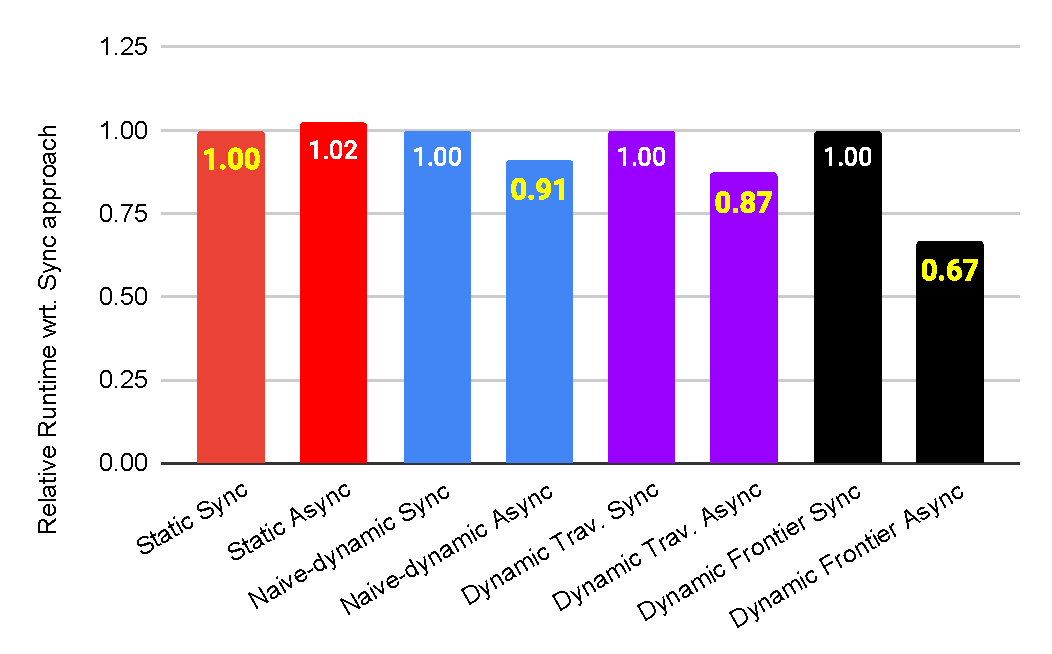
\includegraphics[width=0.48\linewidth]{out/approach-async-mean.pdf}
  }
  \subfigure{
    \label{fig:approach-async--batch}
    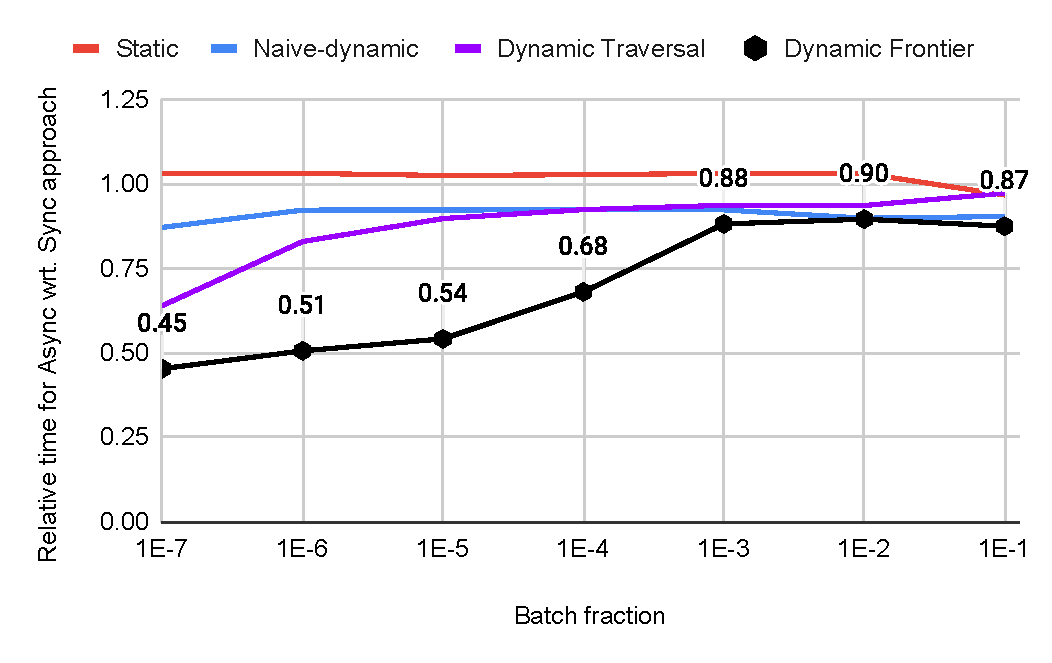
\includegraphics[width=0.48\linewidth]{out/approach-async-batch.pdf}
  } \\[-2ex]
  \caption{Average Relative runtime with asynchronous implementations of \textit{Static}, \textit{Naive-dynamic}, \textit{Dynamic Traversal}, and \textit{Dynamic Frontier} approach compared to their respective synchronous implementations, on batch updates of size $10^{-7}|E|$ to $0.1|E|$ (right), and overall (left). The results indicate that asynchronous implementations are faster than synchronous ones, especially for smaller batch sizes. This is due to a somewhat faster convergence and the absence of copy overhead (for \textit{Dynamic Traversal} and \textit{Dynamic Frontier} approaches).}
  \label{fig:approach-async}
\end{figure*}

\begin{figure}[!hbt]
  \centering
  \subfigure{
    \label{fig:adjust-frontier--runtime}
    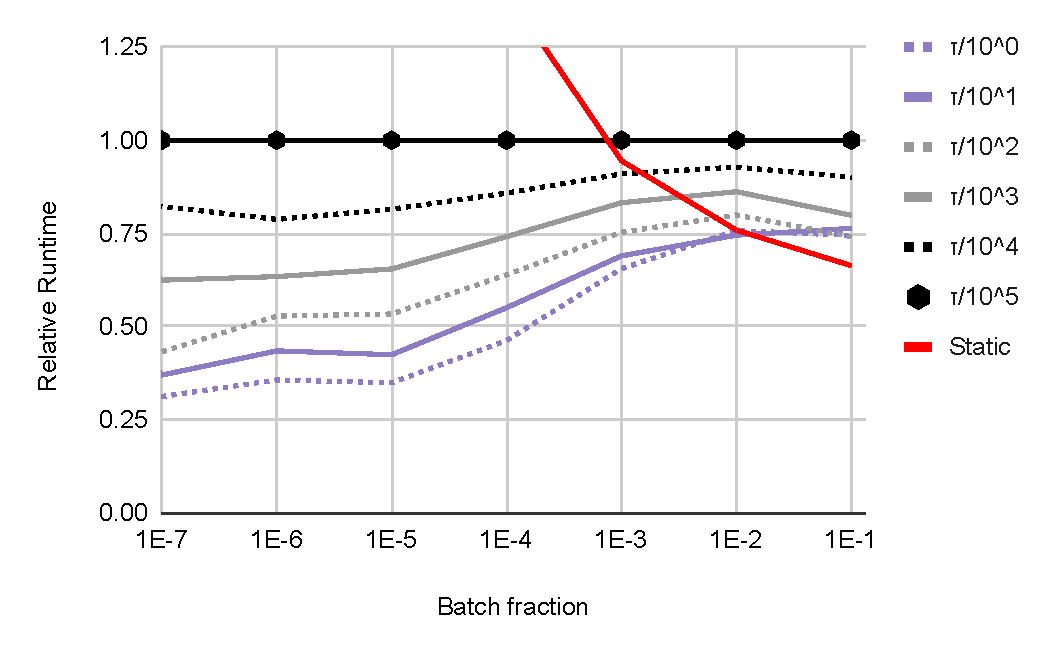
\includegraphics[width=0.98\linewidth]{out/adjust-frontier-runtime.pdf}
  } \\[-1ex]
  \subfigure{
    \label{fig:adjust-frontier--error}
    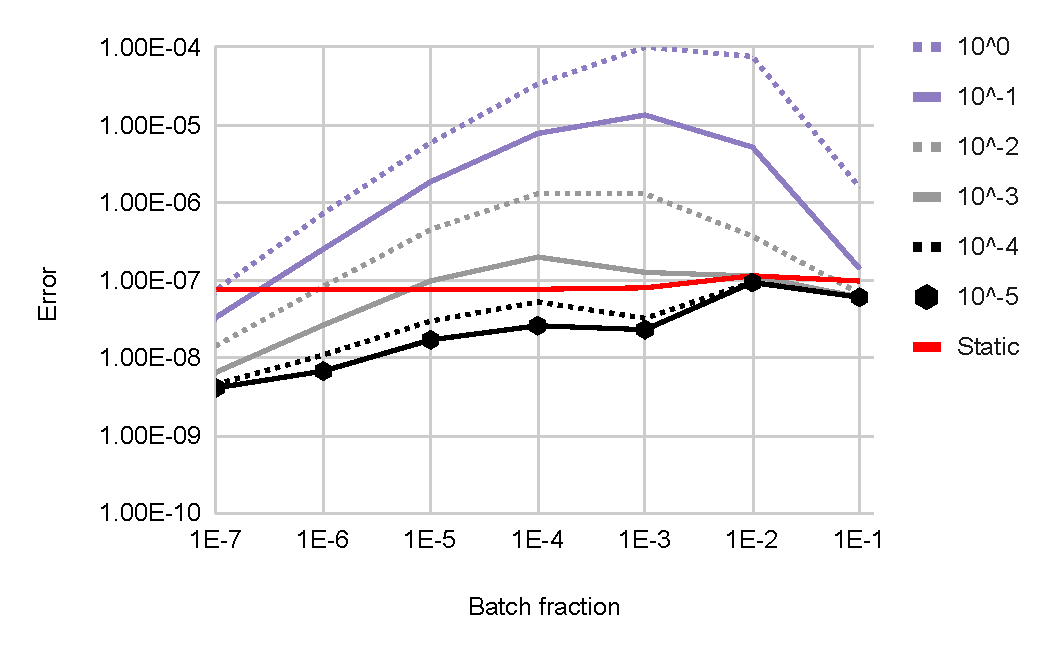
\includegraphics[width=0.98\linewidth]{out/adjust-frontier-error.pdf}
  } \\[-2ex]
\caption{Adjust Frontier. The error is averaged over the graphs in Table \ref{tab:dataset}.}
  \label{fig:adjust-frontier}
\end{figure}





% Dynamic Frontier (DF) approach
% Adjusting tolerance, Frontier tolerance, Mark DelRank / DelContrib
% Dynamic Frontier optimizations
% Edge-balanced approach (Chunk size)
